\chapter{Environment Representation}
\label{chp:Envir-Rep}


%%%%%%%%%%%%%%%%%%%%%%%%%%%%%%%%%%%%%%%%%%%%%%%%%%%%%%%%%%%%%%%%%%%%%%%
\section{Background}
% TODO: Justify why you chose offline

The goal of this paper is to develop a coverage path planning algorithm \hbox{applicable} in a \acl{sar} situation. The goal is for it to be implementable using \acsp{uav}, which can execute three dimensional movements. In this paper however, it is assumed that altitude changes are not necessary to search an area. Assuming that there is some form of camera on-board the \acs{uav}, a constant altitude will be an advantage. It means that the \acf{gsd} will remain constant, which is a widely accepted measure of camera accuracy. Assuming a camera is on a \acs{uav} pointing down towards the ground, \acs{gsd} is the distance on the ground as represented by the width of one pixel \cite{PropellerAero2021}.

Without altitude changes, \acs{uav} motions can be represented in two-dimensional space, which greatly simplifies the problem. For coverage path planning, it is important to have some demarcated two-dimensional region that requires coverage. The identified region, or environment, needs to be represented in either a discrete or continuous manner. 

In the context of \acs{sar}, complete coverage is very important. It will ensure that every possible point in the environment map is covered. In this scenario, it implies that the camera will have viewed all points on the map. Achieving completeness is by no means trivial, but is more achievable in complex environments when using a discrete approach. 
% TODO: Mention drawbacks of continuous implementations
% TODO: Mention reasons for choosing discrete - wavefront planner paper pg 674 "An exact cell decomposition is ineffiecient because we are interested in acquiring an equally sized set of images"

Discretising the environment can be done in a few different ways. Assuming a generic \acs{uav} with some thermal or visual camera on-board, one has a few options. One can discretise the area based on the \acs{uav} size, but a more common practice is to base it off the tool size. In this case, that would be the \acf{fov} of the on-board camera. This also makes the process of complete coverage easier, because if the camera is guaranteed to see the entirety of each discrete cell, it is a complete algorithm so long as each cell is visited.

Therefore, to discretise the environment, the \acl{fov} needs to be calculated. The camera specifications and \acs{uav} altitude will be the determining factors to calculate the \acs{fov}. The type of camera and the flight altitude are design decisions and will depend on the \acs{gsd} necessary to realistically be able to locate the target in a \acl{sar} operation.

The diagram in figure \ref{fig:FOV} shows all the relevant variables needed to calculate the \acl{fov} along one dimension ($FOV_x$). A similar diagram can be used to calculate the \acl{fov} along the other dimension ($FOV_y$). The only difference would be the sensor size variable, which changes from the sensor width ($w_{len}$) to the sensor height ($h_{len}$). The other variables include the focal length of the camera ($f$), the height of the lens above ground ($H$) and the camera's angle of view ($AOV$). Lastly, there is the variable $\phi$ which is an angle created due to the sensor being slightly smaller than the diameter of the cone of light projected onto it.

The resulting \acl{fov} will be a rectangle of the same aspect ratio of the camera sensor, provided the camera is pointing directly down and the ground is level. For this application, it is assumed the camera is always pointing downwards. This can be accomplished when the \acs{uav} banks by placing the camera on a gimble. The assumption that the ground is level is not entirely reasonable, for example, in a mountainous region. This can be addressed by adding overlap between images to add some redundant coverage, which will be added in \ref{chp:refuelling}. Doing a topographical inspection is beyond the scope of this project and will not be addressed in more detail.
% TODO: Check this reference and decide whether to include last sentence

The calculations required to do a discretisation based on the camera \acl{fov} will now be discussed. The first equation that is required is the calculation of the angle $\phi$:\\
\begin{equation}
	\label{eqn:phi}
	\begin{aligned}
		\tan{\phi} &= \frac{\frac{1}{2}w_{len}}{f} &\\
		\phi &= \tan^{-1}{(\frac{w_{len}}{2f})}
	\end{aligned}	
\end{equation}

\tikzset{every picture/.style={line width=0.75pt}} %set default line width to 0.75pt          
\begin{figure}[h!]
	\centering	      
	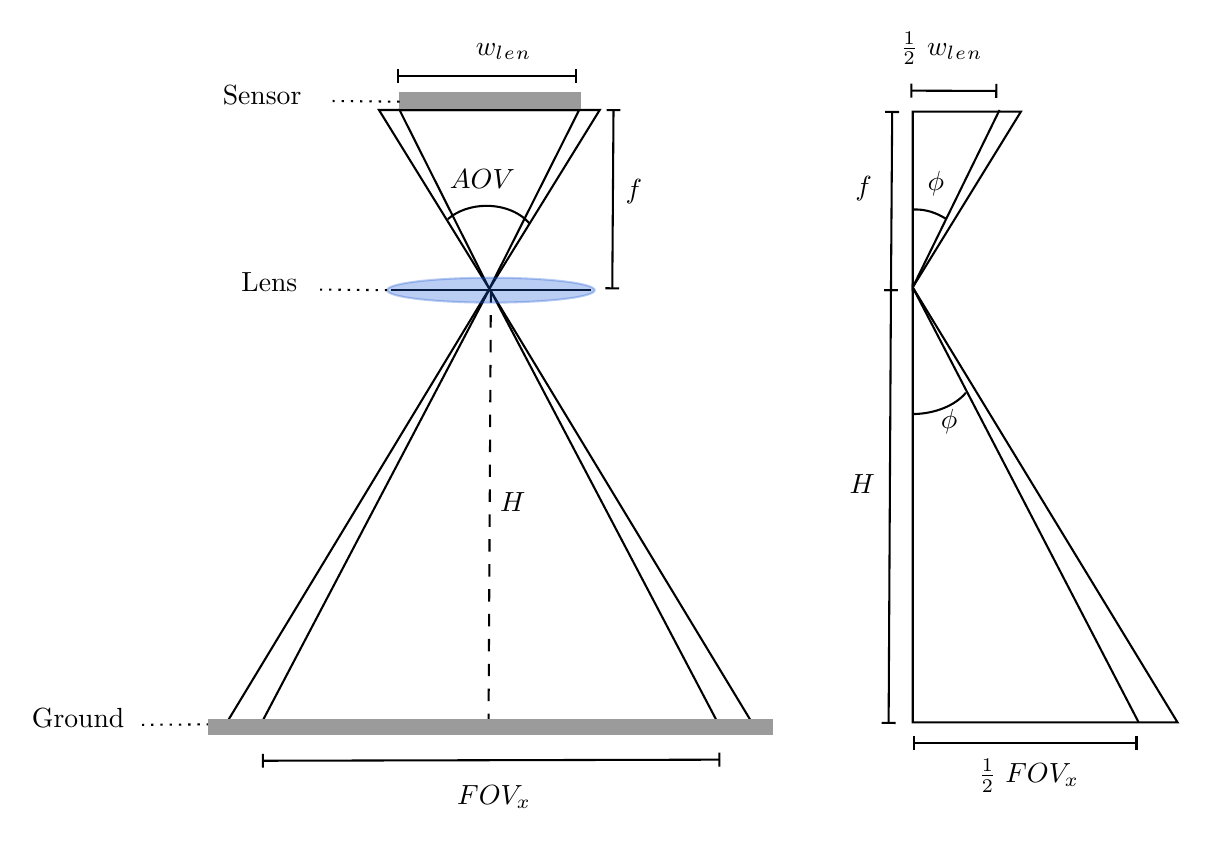
\begin{tikzpicture}[x=0.75pt,y=0.75pt,yscale=-1,xscale=1]
		%uncomment if require: \path (0,445); %set diagram left start at 0, and has height of 445
		
		%Shape: Triangle [id:dp7279031821934365] 
		\draw   (292.52,162.29) -- (239.35,76.17) -- (345.69,76.17) -- cycle ;
		%Shape: Triangle [id:dp08500924272014787] 
		\draw   (292.52,162.29) -- (419.57,372.17) -- (165.48,372.17) -- cycle ;
		%Straight Lines [id:da9387157545116658] 
		\draw    (245.26,162.97) -- (341.26,162.97) ;
		%Shape: Triangle [id:dp15441481766796317] 
		\draw   (292.52,162.29) -- (249.26,76.17) -- (335.78,76.17) -- cycle ;
		%Shape: Triangle [id:dp8187279481172025] 
		\draw   (292.69,162.29) -- (403,372.17) -- (182.39,372.17) -- cycle ;
		%Straight Lines [id:da06491692932377724] 
		\draw    (248.39,59.69) -- (334.14,59.69) ;
		\draw [shift={(334.14,59.69)}, rotate = 180] [color={rgb, 255:red, 0; green, 0; blue, 0 }  ][line width=0.75]    (0,3.35) -- (0,-3.35)   ;
		\draw [shift={(248.39,59.69)}, rotate = 180] [color={rgb, 255:red, 0; green, 0; blue, 0 }  ][line width=0.75]    (0,3.35) -- (0,-3.35)   ;
		%Straight Lines [id:da8254572040663344] 
		\draw    (352.34,76.22) -- (351.75,162.07) ;
		\draw [shift={(351.75,162.07)}, rotate = 270.39] [color={rgb, 255:red, 0; green, 0; blue, 0 }  ][line width=0.75]    (0,3.35) -- (0,-3.35)   ;
		\draw [shift={(352.34,76.22)}, rotate = 270.39] [color={rgb, 255:red, 0; green, 0; blue, 0 }  ][line width=0.75]    (0,3.35) -- (0,-3.35)   ;
		%Straight Lines [id:da18153445552160163] 
		\draw  [dash pattern={on 4.5pt off 4.5pt}]  (293.26,162.97) -- (292.13,371.48) ;
		%Shape: Right Triangle [id:dp9464990257102419] 
		\draw   (548.64,76.92) -- (496.5,161.6) -- (496.5,76.94) -- cycle ;
		%Straight Lines [id:da9593228177444686] 
		\draw    (496.5,161.6) -- (538.33,76.17) ;
		%Shape: Arc [id:dp3427993390498929] 
		\draw  [draw opacity=0] (496.65,124.11) .. controls (496.93,124.1) and (497.22,124.09) .. (497.5,124.09) .. controls (502.76,124) and (507.83,125.61) .. (512.56,128.62) -- (498.77,204.83) -- cycle ; \draw   (496.65,124.11) .. controls (496.93,124.1) and (497.22,124.09) .. (497.5,124.09) .. controls (502.76,124) and (507.83,125.61) .. (512.56,128.62) ;
		%Straight Lines [id:da5534147172451449] 
		\draw    (495.86,66.85) -- (536.76,66.97) ;
		\draw [shift={(536.76,66.97)}, rotate = 180.17] [color={rgb, 255:red, 0; green, 0; blue, 0 }  ][line width=0.75]    (0,3.35) -- (0,-3.35)   ;
		\draw [shift={(495.86,66.85)}, rotate = 180.17] [color={rgb, 255:red, 0; green, 0; blue, 0 }  ][line width=0.75]    (0,3.35) -- (0,-3.35)   ;
		%Straight Lines [id:da49349314045709525] 
		\draw    (486.61,77.11) -- (486.02,162.96) ;
		\draw [shift={(486.02,162.96)}, rotate = 270.39] [color={rgb, 255:red, 0; green, 0; blue, 0 }  ][line width=0.75]    (0,3.35) -- (0,-3.35)   ;
		\draw [shift={(486.61,77.11)}, rotate = 270.39] [color={rgb, 255:red, 0; green, 0; blue, 0 }  ][line width=0.75]    (0,3.35) -- (0,-3.35)   ;
		%Shape: Arc [id:dp09088039941092019] 
		\draw  [draw opacity=0] (272.52,128.74) .. controls (277.02,124.82) and (283.7,122.33) .. (291.17,122.33) .. controls (300.03,122.33) and (307.8,125.84) .. (312.1,131.09) -- (291.17,140.58) -- cycle ; \draw   (272.52,128.74) .. controls (277.02,124.82) and (283.7,122.33) .. (291.17,122.33) .. controls (300.03,122.33) and (307.8,125.84) .. (312.1,131.09) ;
		%Shape: Right Triangle [id:dp9191394953697831] 
		\draw   (496.5,161.6) -- (624.06,371.17) -- (496.5,371.17) -- cycle ;
		%Straight Lines [id:da9606752421348479] 
		\draw    (605.33,371.17) -- (496.5,161.6) ;
		%Shape: Arc [id:dp6813474716985082] 
		\draw  [draw opacity=0] (522.1,212.41) .. controls (516.97,218.5) and (507.3,222.62) .. (496.19,222.67) -- (496,202.42) -- cycle ; \draw   (522.1,212.41) .. controls (516.97,218.5) and (507.3,222.62) .. (496.19,222.67) ;
		%Straight Lines [id:da806740169220673] 
		\draw    (183.39,389.69) -- (403.33,389.17) ;
		\draw [shift={(403.33,389.17)}, rotate = 539.86] [color={rgb, 255:red, 0; green, 0; blue, 0 }  ][line width=0.75]    (0,3.35) -- (0,-3.35)   ;
		\draw [shift={(183.39,389.69)}, rotate = 539.86] [color={rgb, 255:red, 0; green, 0; blue, 0 }  ][line width=0.75]    (0,3.35) -- (0,-3.35)   ;
		%Straight Lines [id:da8133225602503578] 
		\draw    (497.33,381.17) -- (604.33,381.17) ;
		\draw [shift={(604.33,381.17)}, rotate = 180] [color={rgb, 255:red, 0; green, 0; blue, 0 }  ][line width=0.75]    (0,3.35) -- (0,-3.35)   ;
		\draw [shift={(497.33,381.17)}, rotate = 180] [color={rgb, 255:red, 0; green, 0; blue, 0 }  ][line width=0.75]    (0,3.35) -- (0,-3.35)   ;
		%Straight Lines [id:da25053349814928394] 
		\draw    (486.02,162.96) -- (484.89,371.47) ;
		\draw [shift={(484.89,371.47)}, rotate = 270.31] [color={rgb, 255:red, 0; green, 0; blue, 0 }  ][line width=0.75]    (0,3.35) -- (0,-3.35)   ;
		\draw [shift={(486.02,162.96)}, rotate = 270.31] [color={rgb, 255:red, 0; green, 0; blue, 0 }  ][line width=0.75]    (0,3.35) -- (0,-3.35)   ;
		%Shape: Rectangle [id:dp5196090784877698] 
		\draw  [color={rgb, 255:red, 155; green, 155; blue, 155 }  ,draw opacity=1 ][fill={rgb, 255:red, 155; green, 155; blue, 155 }  ,fill opacity=1 ] (249.26,68.14) -- (336,68.14) -- (336,75.17) -- (249.26,75.17) -- cycle ;
		%Shape: Ellipse [id:dp39537204861922115] 
		\draw  [color={rgb, 255:red, 26; green, 88; blue, 211 }  ,draw opacity=0.3 ][fill={rgb, 255:red, 26; green, 88; blue, 211 }  ,fill opacity=0.3 ] (243.26,162.97) .. controls (243.26,159.66) and (265.64,156.97) .. (293.26,156.97) .. controls (320.87,156.97) and (343.26,159.66) .. (343.26,162.97) .. controls (343.26,166.29) and (320.87,168.97) .. (293.26,168.97) .. controls (265.64,168.97) and (243.26,166.29) .. (243.26,162.97) -- cycle ;
		%Shape: Boxed Line [id:dp7067135001640237] 
		\draw  [dash pattern={on 0.84pt off 2.51pt}]  (243.26,162.97) -- (211,162.67) ;
		%Straight Lines [id:da962687715126145] 
		\draw  [dash pattern={on 0.84pt off 2.51pt}]  (157.48,372.17) -- (125.22,372.37) ;
		%Shape: Boxed Line [id:dp25644897900816477] 
		\draw  [dash pattern={on 0.84pt off 2.51pt}]  (249.26,72.14) -- (217,71.84) ;
		%Straight Lines [id:da9121328450253205] 
		\draw [color={rgb, 255:red, 155; green, 155; blue, 155 }  ,draw opacity=1 ][line width=6]    (157.17,373.35) -- (429.09,373.35) ;
		
		% Text Node
		\draw (277.85,37.29) node [anchor=north west][inner sep=0.75pt]  [font=\normalsize]  {$ \begin{array}{l}
				w_{l}{}_{e}{}_{n}\\
			\end{array}$};
		% Text Node
		\draw (171.59,152.9) node [anchor=north west][inner sep=0.75pt]  [font=\normalsize] [align=left] {Lens};
		% Text Node
		\draw (356.67,108.27) node [anchor=north west][inner sep=0.75pt]  [font=\normalsize]  {$f$};
		% Text Node
		\draw (296.25,259.08) node [anchor=north west][inner sep=0.75pt]  [font=\normalsize]  {$H$};
		% Text Node
		\draw (272.06,103.36) node [anchor=north west][inner sep=0.75pt]  [font=\normalsize]  {$AOV$};
		% Text Node
		\draw (502.19,104.3) node [anchor=north west][inner sep=0.75pt]  [font=\normalsize]  {$\phi $};
		% Text Node
		\draw (467.33,106.6) node [anchor=north west][inner sep=0.75pt]  [font=\normalsize]  {$f$};
		% Text Node
		\draw (489,37) node [anchor=north west][inner sep=0.75pt]    {$\frac{1}{2} \ w_{l}{}_{e}{}_{n}$};
		% Text Node
		\draw (508.52,218.96) node [anchor=north west][inner sep=0.75pt]  [font=\normalsize]  {$\phi $};
		% Text Node
		\draw (268.85,398.07) node [anchor=north west][inner sep=0.75pt]  [font=\normalsize]  {$ \begin{array}{l}
				FOV_{x}\\
			\end{array}$};
		% Text Node
		\draw (520,387.4) node [anchor=north west][inner sep=0.75pt]  [font=\normalsize]  {$ \begin{array}{l}
				\frac{1}{2} \ FOV_{x}\\
			\end{array}$};
		% Text Node
		\draw (464.59,250.41) node [anchor=north west][inner sep=0.75pt]  [font=\normalsize]  {$H$};
		% Text Node
		\draw (162.59,62.9) node [anchor=north west][inner sep=0.75pt]  [font=\normalsize] [align=left] {Sensor};
		% Text Node
		\draw (70.59,363) node [anchor=north west][inner sep=0.75pt]  [font=\normalsize] [align=left] {Ground};
		
		
	\end{tikzpicture}
	\caption{Diagram showing relevant variables concerned with calculating the Field of View for a camera.}
	\label{fig:FOV}
\end{figure}
